%  Copyright 2020-2022 Robert Bosch GmbH
%
%  Licensed under the Apache License, Version 2.0 (the "License");
%  you may not use this file except in compliance with the License.
%  You may obtain a copy of the License at
%
%      http://www.apache.org/licenses/LICENSE-2.0
%
%  Unless required by applicable law or agreed to in writing, software
%  distributed under the License is distributed on an "AS IS" BASIS,
%  WITHOUT WARRANTIES OR CONDITIONS OF ANY KIND, either express or implied.
%  See the License for the specific language governing permissions and
%  limitations under the License.
\chapter{Code analysis}

The \rfw\ installation provides a static code analyser to detect potential errors and violations to coding conventions.
The name of the analyser is \textbf{Robocop}.

Robocop is integrated in Visual Studio Code and and is triggered automatically in case of
\begin{enumerate}
   \item a file is opened in editor,
   \item a file is changed and saved.
\end{enumerate}

The outcome will look like this:

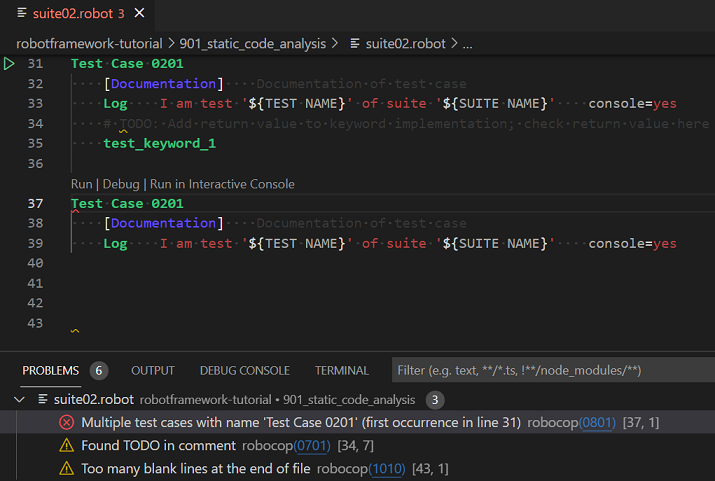
\includegraphics{./include/graphics/code_analysis/Overview}

Further examples can be found in the \rfw\ tutorial, chapter \rlog{901_static_code_analysis}.

\vspace{2ex}

\textbf{How to configure?}

Robocop contains a set of rules that are used to check the source files of the \rfw. Not all of them are really useful and some of them are also against
our company internal development rules. Therefore we have the need to exclude rules from Robocop execution.

Some rules can be configured (e.g. the rule checking the maximum number of characters within a line of code). Also here we have the need for careful adaptions.

When Robocop is triggered automatically within Visual Studio Code, then the configuration is done with the help of a \rlog{.robocop} file. This file has to be placed 
within the projects folder (see tutorial). To make Robocop results comparable this configuration file should not be modified - or at least should be kept aligned with
the version all other project team members use.

\newpage

\textbf{Command line}

In addition to the automated triggering within Visual Studio Code Robocop can also be called in command line. This is useful
\begin{enumerate}
   \item in case of a complete folder has to be checked in one step (to avoid the need to open every single source file inside separately),
   \item in case of an alternative configuration is wanted (temporarily; to avoid to manipulate the standard configuration file),
   \item in case of Robocop shall be triggered by automats like Jenkins,
   \item in case of the Robocop results are needed within a log file (output to a log file needs to be configured separately).
\end{enumerate}

To give it a try make a copy of the configuration file \rlog{.robocop} available within the tutorial, and give this copy any other name (e.g. \rlog{robocop.arg}).

Now Robocop can be called with command lines like this:

\vspace{2ex}

\textit{1.) Simple check of single file with default configuration:}

\begin{pythoncode}
"%RobotPythonPath%/python.exe" -m robocop "<\inlinecomment{path}>/mytestfile.robot"
\end{pythoncode}

\vspace{2ex}

\textit{2.) Check of single file with individual configuration taken from argument file:}

\begin{pythoncode}
"%RobotPythonPath%/python.exe" -m robocop --argumentfile "<\inlinecomment{path}>/robocop.arg" "<\inlinecomment{path}>/mytestfile.robot"
\end{pythoncode}

\vspace{2ex}

\textit{3.) Check of entire folder with individual configuration taken from argument file:}

\begin{pythoncode}
"%RobotPythonPath%/python.exe" -m robocop --argumentfile "<\inlinecomment{path}>/robocop.arg" "<\inlinecomment{folder}>"
\end{pythoncode}

\vspace{2ex}

\textbf{How to activate?}

In Visual Studio Code the automated triggering of Robocop is activated per default within

\begin{robotlog}
RobotFramework\robotvscode\data\user-data\User\settings.json
\end{robotlog}

with the following switches set to \rcode{true}:

\begin{pythoncode}
"robot.lint.enabled": true,
"robot.lint.robocop.enabled": true,
\end{pythoncode}

